
%\documentclass[9pt]{article}
\documentclass[9pt,twocolumn]{article}
\setlength{\columnsep}{.35in}
\usepackage[pdftex]{graphicx}
\usepackage[top=2in, bottom=1.5in, left=.7in, right=.7in]{geometry}
\usepackage{booktabs}
\usepackage{array}
\usepackage{amsmath}
\usepackage{subfigure}
\usepackage{epstopdf}

\begin{document}
\setlength{\parindent}{0cm}

\fontencoding{T1}
\fontfamily{Arial}\selectfont
%\fontfamily{Times New Roman}\selectfont
\fontseries{m}
\fontsize{10}{10}\selectfont

\title{}
\author{ }
\date{}
\maketitle

\section*{Abstract}

A novel approach is presented to efficiently and accurately identify intersections between pairs of rigid nonconvex bodies and compute the contact points and associated normals of the intersecting regions. Starting from the signed distance filed approach to collision detection, we show how it can be modified in order to obtain accurate contact point/normals information as well as made efficient and robust to the cases of edge-edge and face-face contact. We demonstrate through a number of scenes that our scheme produces accurate contact points/normals and is as fast for general convex rigid bodies and significantly faster for concave bodies than the popular GJK algorithm.

\section{Introduction} 

A key aspect of physical simulation of rigid and deformable bodies is collision detection. Collision detection may be classified into discrete and continuous schemes. In discrete schemes, the physical simulation is advanced from some time $t_0$ to time $t_1 = t_0 + \Delta t$ after which an interference query is performed. Inherently, this leaves open the possibility that two bodies\footnote{Throughout the rest of this paper, rigid bodies will be referred to as just bodies.} do not collide at times $t_0, t_1$ but collide at some time on the interval $[t_1, t_2]$. A second but more troubling difficulty occurs with the construction of the contact manifold. Central to this difficulty is deciding on a set of points and normals to represent it accurately. \newline

In contrast to discrete collision detection schemes, continuous schemes seek to find the exact time $t \in [t_0, t_1]$ when the collision occurs. Beyond the obvious advantage that collisions cannot be missed, determination of contact points and normals for the contact manifold becomes straightforward. Specifically, the set of contact points are those locations in which the separation distance is zero. In the case of smooth manifold geometry, colliding surfaces define coplanar tangent planes at the contact points. The contact normal may be taken as the normal of either plane up to a sign. Although not quite as straightforward, a similar definition of contact normals may be defined for polygonal geometry. Despite these advantages, continuous collision detection can be orders of magnitudes slower than discrete schemes in complex simulation. As a result, discrete schemes are used for complex real-time simulations and methods have been developed to lessen their deficiencies. In most situations, collisions will not be completely missed, so most work has been directed towards methods of computing the contact manifold.\newline

A geometric standpoint may be taken with the contact points/normals determined by closest features or contact types (i. e. vertex-vertex, vertex-edge, etc.). Efficient methods to determine closest features usually involve feature based algorithms (GJK, V-Clip) which in turn assume the bodies being dealt with are convex or composed of convex pieces. Bounding volume hierarchies present an alternative not tied to convexity, yet they are unable to efficiently compute closest features and instead rely on contact types to determine contact points/normals. In the end, neither closest features nor contact types are sufficient for determining correct contact points/normals for convex or concave bodies when there is deep penetration. \newline

The situation of deeply penetrating bodies may be handled better by a distance based approach. In these schemes, a signed distance function defined on a volume enclosing the body is computed. Possible contact points may be checked by direct evaluation of the signed distance function and the contact normals computed from the gradient of the function. Distance based schemes are more robust to deeper penetration; nonetheless, the gradient may be faulty in indicating the direction of the desirable contact normal (Figure 3). These approaches also are unable to handle edge-edge collisions efficiently; solutions that exist end up over generating contact points or relying on completely different schemes. Furthermore, face-face contact can be problematic as illustrated in Figure 1. \newline

The final class of schemes relies on a volume based approach. Instead of considering the contact manifold as a 2D surface, these approaches consider it as a 3D volume. Layered depth images (LDI's) are used to compute the intersection volumes. After which, repulsion forces or contact constraints are formulated upon these volumes. The directions of these forces or constraints act in the direction of the ``pressure force'' generated by the contact volume.  These schemes do not require any precomputed data, are suitable to rigid and deformable bodies, and are robust to even deeper penetration than distance based approaches. However, LDI's are only applicable to GPU computation, thus limiting these approaches to the GPU. In addition, it is unclear how well these schemes work for very large scenes as the size of the LDI's may need to be exceedingly large. \newline

We present an extension to the signed distance field approach that resolves the problem of faulty contact normals using the concept of admissible zones\cite{English} as well as a new approach to resolve the edge-edge and face-face cases without resorting to a separate scheme or over generating contact points. Faulty contact points/normals are dealt with through the concept of  admissible zones. A set of possible contacts is generated based upon sampling the various features of a body: vertices, edges, and faces. The various features are sampled to result in a minimum set that can still represent the contact manifold accurately and robustly; guaranteeing this amounts to placing a restriction on the maximum linear and angular velocity that a body can have. Depending on which feature the contact  location was generated from, a different routine is employed to check if the contact location is valid and if so compute a contact normal. Through these measures we are able to efficiently and robustly handle the cases of edge-edge and face-face contact in a unified framework.  We implement our approach for the CPU  and demonstrate the accuracy on several difficult scenes and show its improved performance for concave bodies when compared with GJK as implemented by Bullet.

\section{Related Work}

The degree of work on collision detection is rather vast and for a survey of the various approaches in general, we refer the reader to the excellent surveys of \cite{Lin} and \cite{Teschner}. We may, however, give an overview of what works strictly apply to generating robust and physically plausible contact points/normals, for there is surprisingly little effort in this area. As mentioned previously, geometric methods make direct use of the geometry for collision detection. Perhaps, the archetypal scheme is the bounding volume hierarchy (BVH), see \cite{Gottschalk}, \cite{Hubbard}. As far as we are aware, the only work that, addresses contact point/normal generation specifically for BVH is \cite{Erlebenetal}. For each pair of intersecting triangles that a BVH returns, \cite{Erlebenetal} determine the contact points/normals for that triangle pair by considering the type of contact pair the triangles form, i. e. vertex-vertex, vertex-face, etc. As pointed out by \cite{Erlebenetal}, it may be difficult to decide which contact pair it is exactly, leading to incorrect results if  misclassified. The other common geometric paradigm is the feature based one with the schemes GJK\cite{Gilbert} and V-Clip\cite{Mirtich} the most popular. For two convex bodies, these schemes return the closest features and a maximum penetration depth estimate, but in general they do not return information about the entire contact manifold at a single invocation\cite{Mirtich}.  In Bullet\cite{Coumans} the issue is dealt with by caching contact points over multiple frames of the simulation, resulting in a contact manifold. \newline

The work of \cite{Guendelman} introduced signed distance fields into the realm of rigid body simulation. Their approach is to store for each body an object space discretization of the signed distance function $\phi(x)$ in a uniform grid. $\phi(x)$ can then be approximately reconstructed  by trilinear interpolation of the grid nodes. In addition, the normal at any point $x$ on the body or in space may be calculated as $\nabla \phi(x)$. The details of constructing the signed distance function can be found in \cite{Tsitsiklis}\cite{Sethian}. For collision detection of two bodies, it is then simply a matter of evaluating $\phi(x)$ for each body on sample locations from the other body. The sample locations may be taken as the vertices of the triangular mesh representation of a body \cite{Guendelman}, and whether or not a location, $x$,  is contained is determined by the sign of $\phi(x)$. For each point that is contained, the contact normal is given by $\nabla \phi(x)$. Nonetheless, this approach does not handle the edge-edge and edge-face cases directly as neither vertex of the edge may be contained in the other body, but the edge still intersects on some interior interval. In \cite{ErlebenPhd} the edges are sampled themselves, dealing with this problem but at the same time introducing over sampling. Furthermore, vertex and edge sampling alone may be insufficient to handle nearly identical face-face contact as in Figure~\ref{Problem1} where neither the vertices or edges result in contact normals that are appropriate. \cite{ErlebenPhd} introduces sampling of the faces as well to deal with this situation. \newline

\begin{figure}[ht]
\centering
\subfigure[]{
	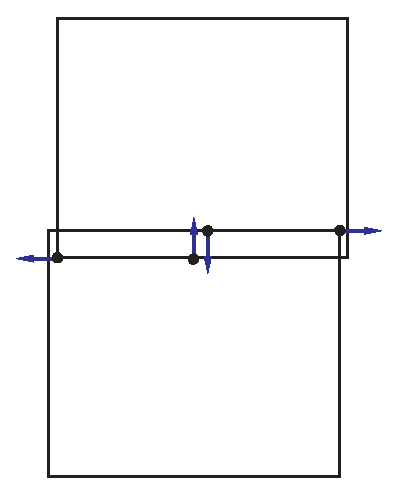
\includegraphics[scale = .68]{Figure_1b.eps}
	\label{fig:subfig1}
}
\subfigure[]{
	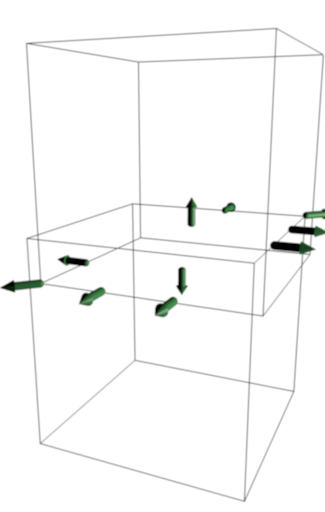
\includegraphics[scale = .68]{Figure_1b.png}
	\label{fig:subfig2}
}
\caption{(a) Side view of two 3D boxes (b) in a box stack colliding with each other under the influence of gravity in the vertical direction. Vertex and edge sampling alone result in contact normals perpendicular to the direction of gravity, allowing for further penetration. Face centroid sampling results in contact normals that oppose the direction of gravity and prevent further penetration. }
\label{Problem1}
\end{figure}

Works by the authors \cite{Vassilev}, \cite{Heidelberger}, \cite{Wong}, \cite{Sud}, \cite{Faure}, \cite{Allard} introduced and considered various paradigms of GPU collision detection. But of particular relevance, are the works of \cite{Faure}, \cite{Allard}, which specifically address the formation of contact points/normals. In these works,  LDI's are used for collision detection and for the construction of a contact volume. The LDI data structure is formed by a stack of textures (layers) in the view direction. Each texture at a given pixel location stores the distance to the object surface as well as additional geometric information. A ray parallel to the view direction through a pixel location can be divided into intervals of intersection by sorting the depths in the LDI's for that pixel location. Determining the intersections requires only one LDI in the view direction; however, it is necessary to construct two more in orthogonal directions to compute the volumes of intersection. For each volume, a contact constraint can be formulated which can be viewed as a constraint on the 3D contact manifold or contact volume instead of constraints on the traditional 2D contact manifold. The directions of these forces or constraints are then chosen to minimize the intersection volume most quickly. Because a single contact constraint per volume is not sufficient to model varying friction and concave bodies, \cite{Allard} describes dividing the contact volume into subvolumes based upon a uniform grid. Constraints are then formed for these subvolumes. 

\section{Admissible Zones}

The admissible zone may be defined as the conical combination of the normals of the face meeting at the feature--that is, a vector for a plane, a wedge for an edge, and an n-sided pyramid for a vertex (Figure~\ref{fig:AdmissibleZone}) \cite{English}. We make a simplification in treating the n-sided pyramid for a vertex as a cone, which is justified in typical situations. Given a body with signed distance field $\phi(x)$, the condition of whether or not a point, $x$, is admissible assuming that this point is already contained in the body can be formulated as 

\begin{equation}
(-\nabla \phi(x)) \cdot k > \delta
\end{equation}
where $\delta$ is the half angle of the admissible cone and $k$ is the vector bisector of the cone. Turning to Figure~\ref{fig:AdmissibleExample}, we see that by discarding non-admissible contact points, a troublesome case can be dealt with.

\begin{figure}[h]
\centering
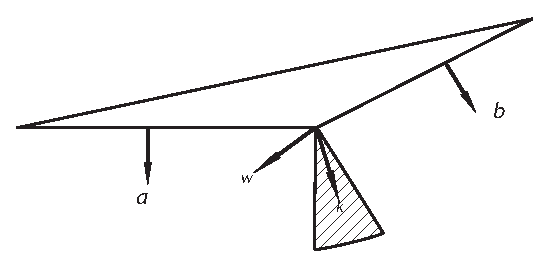
\includegraphics[scale = .85]{AdmissibleZone.eps}

\caption{The face normals $a$, $b$  designate the boundary of the admissible zone. Only vectors lying in the shaded cone are admissible, excluding $w$ from admission. }

\label{fig:AdmissibleZone}
\end{figure}


\begin{figure}[h]
\centering
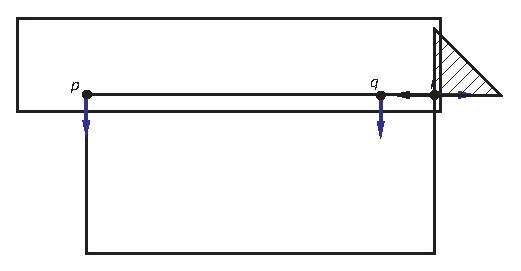
\includegraphics[scale = 1.]{Figure_3.eps}

\caption{The contact normal (blue) at $r$ hinders the two boxes from sliding horizontally against one another. The direction $-\nabla \phi(r)$ does not lie in the admissible zone at $r$, and $r$ can, therefore, be discarded, resolving the issue. On the other hand, the points $p, q$ are certainly admissible and added to the contact manifold. 
}
\label{fig:AdmissibleExample}
\end{figure}

\section{Collision Detection with Signed Distance Fields}

With each body in the simulation, we precompute a signed distance function $\phi(x)$ evaluating to a positive nearest feature distance if $x$ is outside the body and negative if it is contained. In addition, the sets $\Gamma, \ \Omega$ are computed which define sampling locations for each body. The set $\Gamma$ corresponds to samples generated on the vertices where as $\Omega$ corresponds to samples on the faces. We perform collision detection of two bodies by determining which features (vertices, faces, edges), represented by our samples, of the first are contained in second and conversely. We note specifically that a set of edge samples was not precomputed as edges are adaptively sampled. As will be seen below by sampling each feature, the problematic cases mentioned previously are resolved (Figures 1, 3). For the general case of more than two bodies, collision detection becomes the described pairwise evaluation over all possible pairs. Before describing how the samples for each set are precomputed  and collision detection handled for each feature, we need assume that limits on the maximum linear and angular velocities of a body are enforced. By enforcing these limits, it is possible to derive a bound on the maximum penetration depth between two bodies, which is necessary in order to avoid over sampling. It should be noted that simply the time step could have been reduced in order to prevent bodies from penetrating too deeply, but for real-time applications, such a method may significantly hamper the overall speed of the simulation. We now outline sampling and collision detection for each feature for the case of two bodies possibly colliding. \newline

{\bf Vertex Features:} We precompute $\Gamma$ by sampling every vertex and perform collision detection by determining if any samples, $x$,  results in $\phi(x) < 0$. For those samples that satisfy $\phi(x) < 0$, the contact normal is computed from $\nabla \phi(x)$ and if (1) is satisfied, the contact point/normal are added to the contact manifold. \newline

{\bf Face Features:} We can treat collision detection of face features similar to vertex features but using the set of face samples, $\Omega$. It remains then to precompute $\Omega$ that is sufficient to handle the case presented in Figure 1, but does not contain redundant sample locations. We start by noting that face sampling is only necessary in the situation of two identical or nearly identical faces in contact. In highly tessellated bodies, similar faces touching is highly unlikely and even if they do touch and penetrate slightly, there will be sufficient vertices and thus contact points/normals  in the surrounding neighborhood that yield valid contact normals to prevent much penetration. Because of this, we are justified in only sampling regions of lower tessellation. \newline

In Figure~\ref{Figure5}a, the points represent locations leading to admissible contact points, but simply adding all these admissible locations to $\Omega$ will clearly result in redundant contact points. Instead, given a body with $n$ faces, we let $\Omega = \Omega_1 \cup \Omega_2 \cup ... \cup \Omega_n$ where $\Omega_k$ is the convex hull of the set of admissible points on the face, $k$. This would minimize the number of contact points while at the same time still producing an accurate contact manifold. Unfortunately, for different levels of penetration this set varies and $\Omega_k$ could not be precomputed. Nonetheless, we can make a reasonable choice for $\Omega_k$ with a slightly less accurate representation of the contact manifold. That is, we can choose the samples for $\Omega_k$ from the boundary vertices of the convex hull of the set of admissible points when there is maximum penetration (Figure 5b). In any case of lesser penetration, $\Omega_k$ will still be admissible but not completely ideal. We now shall see how this can be formalized precisely. \newline

\begin{figure}[t!]
\centering
\subfigure[]{
	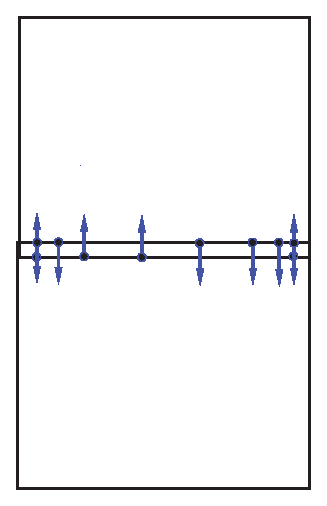
\includegraphics[scale = .7]{Figure_5a.eps}
	\label{fig:subfig1}
}
\subfigure[]{
	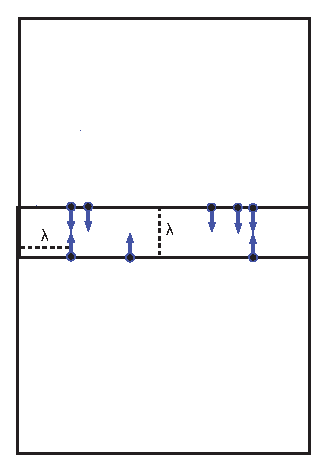
\includegraphics[scale = .7]{Figure_5b.eps}
	\label{fig:subfig2}
}
\subfigure[]{
	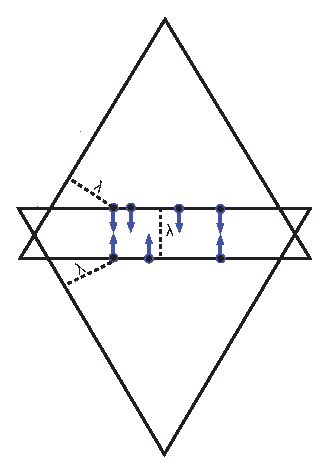
\includegraphics[scale = .8]{Figure_5c.eps}
	\label{fig:subfig2}
}
\caption{A side view of bodies in 3D colliding with each other. Contact points/normals have been drawn in admissible locations. In (b) the valid contact points/normals  are inset substantially compared to those of (a). Nonetheless, any contact point/normal in (b) is certainly valid for (a). A larger inset of the vertices is required in the case of the triangular shaped objects of (c). }
\label{PenetrationDist1}
\end{figure}

It is first necessary to find the maximum penetration between two objects. From the maximum linear velocity, $\nu^{max}$, the maximum linear penetration distance is $\lambda^{\nu} =  ||\nu^{max}|| \Delta t$ where $\Delta t$ is the time step. To take into account the angular velocity, we linearize, yielding a  linear velocity. Unfortunately, we now have a dependency on the shape of the body, or to be more specific, the linearized angular velocity depends upon the distance from a particular location to the center of mass of the body. For a face $k$ with vertex $i$ of it, the maximum angular penetration distance is $\lambda_{k,i}^\omega = ||\omega_{k,i}|| \Delta t$ with $\omega_{k,i}$ the linearized angular velocity. This gives the maximum penetration for a vertex of a face as $\lambda_{k,i} = \lambda^\nu + \lambda_{k,i}^{\omega}$. With this distance defined, the set of points defining the convex hull can be found by "insetting" the vertices of a face based upon the the maximum penetration distance for each vertex. \newline

\begin{figure}[t]
\centering
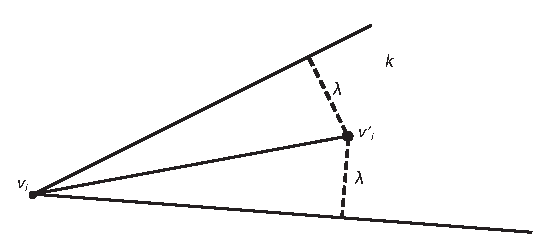
\includegraphics[scale = .84]{Figure_4a.eps}
\caption{Here, for vertex $i$ on face $k$, the inset vertex $v_i'$ is inset by the maximum penetration distance $\lambda$.}
\label{PenetrationDist2}
\end{figure}

Viewing Figure 4, it can be seen that the locations that are always admissible on a face are those that are inset by the maximum penetration distance from the sides of that face. Figure 5 provides a top view of a face, $k$, in which we assume that the edges of face $k$ make a 90 degree dihedral angle w.r.t. to the face (Figure (b)). The location of the inset vertex is $v_{k,i}'$, which is $v_{k,i}$ inset by $\lambda_{k,i}$ from both its edges. Given a successively ordered list of vertices of face $k$ as $(v_{1,k}, v_{2,k}, ...)$, a formula for the inset vertex can be given as

\begin{equation}
v_{k,i}' = \frac{\lambda_{k,i}}{|| e_{k,i}^1 \times (e_{k,i}^1 + e_{k,i}^2)||}\frac{e_{k,i}^1 + e_{k,i}^2}{\|(e_{k,i}^1 + e_{k,i}^2),\|},
\end{equation}
where
\begin{equation*}
 e_{k,i}^1 = \frac{v_{i-1,k} - v_{i,k}}{||v_{i-1,k} - v_{i,k}||}, e_{k,i}^2 = \frac{v_{i+1,k} - v_{i,k}}{||v_{i+1,k} - v_{i,k}||}
\end{equation*}
Extending this for dihedral angles less than 90 (Figure (c)) is straightforward, and we omit further details. It should be noticed that it is certainly possible that an inset vertex lies outside the face that it belongs to in which case the inset vertex is simply discarded. But this is exactly what we were seeking for a sampling method. For small triangles, all the inset vertices will be discarded since they are not necessary where as for large triangles a set of inset vertices will exist. \newline

{\bf Edge Features:} We let an edge be denoted by its two endpoints which without loss of generality are denoted $v^1, v^2$. In addition, let $e^1 = v^2 - v^1, e^2 = v^1 - v^2$ be the edge directions, and $\phi(v^1), \phi(v^2)$ be the signed distances of the closest points on the other body to $v^1, \ v^2$, respectively. For collision detection, we begin by considering if $\phi(v^1), \phi(v^2) > 0$ and $\phi(v^1) + \phi(v^2) \ge \|v^2 - v^1\|$, then the edge may be discarded as no point on this edge can satsify $\phi(x) < 0$. Otherwise, we would like to find the region of intersection. Our method does not guarantee that this region will always be found; it would be prohibitive in terms of cost to guarantee this. Nonetheless, the method makes a guarantee on the maximum distance that two edges can penetrate each other. \newline

Our method begins by first contracting the edge in order to quickly discard a possibly large region that cannot contain the region of intersection. Since $\phi(v^i) > 0$ implies that $\phi(x)$ cannot be negative at least within the ball of radius $\phi(v^l)$, the endpoint $v^i$ can be contracted to $v^i = v^i - \phi(v^i) \cdot \frac{v^i}{\|v^i\|}$. Now, a check for containment with a set of uniform samples on the contracted edge is made, discarding the edge if none are contained. The distance between samples is proportional to the maximum distance, $d_s$ two lines initially touching can separate after one time step given zero initial velocity and an acceleration due to gravity. We see in Figure 6a a set of samples with sampling distance given by $d_s$. In 6b this distance must be reduced because of the dihedral angle of the edge. The sampling distance can be given as $2\tan(\theta) d_s$ where $\theta$ is the half dihedral angle of the edge. Although for each edge we could compute a sampling distance based upon its  angle, it is meaningless unless the discretized signed distance field is fine enough to capture the edge. Furthermore, in all of our tests, taking the sampling distance uniformly as just $2 d_s$ resulted in unnoticeable edge-edge penetrations. \newline

\begin{figure}[ht!]
\centering
\subfigure[]{
	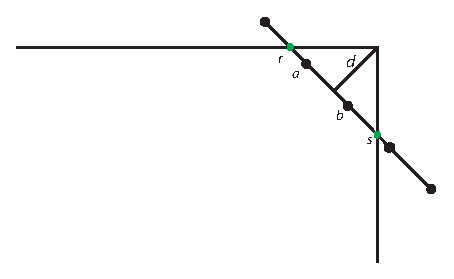
\includegraphics[scale = .8]{Figure_6a.eps}
	\label{fig:subfig1}
}
\subfigure[]{
	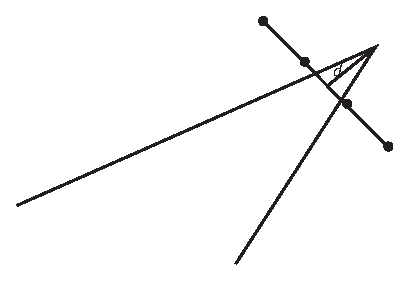
\includegraphics[scale = .8]{Figure_6b.eps}
	\label{fig:subfig2}
}
\caption{A side view of two edges in 3D colliding with each other. In (a) our sampling distance of $d_s$ is sufficient to always find a point of intersection on the edge. The samples closest to the edge end points are labeled as $a, b$, and $r, s$ represent the contact points. (b) The same sampling distance used in (a) is insufficient to find a collision. }
\label{EdgeEdge}
\end{figure}

With sampling frequency of each edge determined, we can find two contact points that best represent it. The samples along the edge are tested for containment ($\phi(x) < 0$). Assuming that the test succeeds, let $s^i$ be the sample closest to edge endpoint $v^i$. 
Although this sample may be closest to the edge endpoint, there may still be considerable distance between the actual face of the other body that this edge intersects with and the sample location (Figure 6a). In order to compute an accurate contact normal, it is necessary that these distances be as small as possible. Because of this consideration, we perform a linear or binary search starting from each closest sample to its corresponding closest endpoint, stopping when we are as close as one grid cell. We take these points that we find as the contact points and denote them $t^1, t^2$. Lastly, it should be noted that the approach outlined here assumes that the other body touches this edge in exactly one region. This is certainly true for convex bodies but may be violated in unusual cases of concave ones. Nonetheless, it is straightforward matter to extend this approach to multiple edge intersections. \newline


%We start at $v^l$ and sample in the direction of $v_i$ until a sample is found such that $\phi(x) < 0$. If no point was found, then the edge is considered non-intersecting and discarded. If not, we let $q_c$ be the contained sample starting from $e_0$ and $q_{nc}$ be the sample right before this. Similarly define $p_c$ and $p_{nc}$ for the endpoint $e_1$. A linear or binary search is performed over $p_c, p_nc$ and $q_c, q_{nc}$ with stopping criteria that $\|p_c - p_{nc}\|, \|q_c - q_{nc}\| \le$ $\alpha \cdot$(cell size of the grid). This gives the two contact points, which are added to the contact manifold, as $t_0 = p_c$ and $t_1 = q_c$. \newline

To determine the contact normals for our contact points, there are three cases that need be considered. If either the endpoints, $v^1$, $v^2$, corresponds to a vertex that is admissible, we set both of the normals for $t^1,t^2$ to be the normal of the admissible endpoint. On the other hand, if neither is admissible, we are left with either an edge-edge or edge-face intersection. If we let $n^1 = \frac{\nabla \phi(t^1)}{\|\nabla \phi(t^1)\|}, n^2 = \frac{\nabla \phi(t^2)}{\|\nabla \phi(t^2)\|}$, then the cases can be distinguished based upon whether or not $n^{1/2} = \frac{\nabla \phi((t^1+t^2)/2)}{\|\nabla \phi((t^1 + t^2)/2)\|}$ is contained in the span of $n^1, n^2$. If $n^{1/2}$ is within the span, then we have an edge-edge intersection. Since we do not know the edge of the other body and hence edge direction of it, it is necessary to find an approximation to this direction. We may compute this approximation as $n^{12} = n^1 \times n^2$. The direction of the contact normal is then simply given as $n^{12} \times e^1$. In the case that $n^{1/2}$ is not contained in the span, we have an edge-face intersection in which $n^{1/2}$ will represent a reasonable approximation to the normal direction of the face. 


\section{Results}

\begin{table*}
\centering
\begin{tabular}{!{\vrule width 2pt}l!{\vrule width 2pt}c|c | c|c | c | c!{\vrule width 2pt}} \noalign{\hrule height 2pt}
	Scene & Objects & Triangles &  Contact Points & Collision Detection & Constraint Solve & Frames Per Second\\ \noalign{\hrule height 2pt}
	Box-Pyramid & 450 & 5.4K &  4.1K & .020s & .009s & 30\\ \hline
	Convex & 200 & 7.2K &  2.2K & .033s & .003s & 24\\ \hline
	Concave Simple & 50 & 5.2K &  700 & .008s & .001s & 24\\ \hline \noalign{\hrule height 2pt}
\end{tabular}
\centering
\caption{Complexity and measured performance of our approach. Timings represent the average time spent in the various parts of the simulation on a per frame basis.}
\label{table1}
\end{table*}

\begin{table*}
\centering
\begin{tabular}{!{\vrule width 2pt}l!{\vrule width 2pt}c|c | c|c | c | c!{\vrule width 2pt}} \noalign{\hrule height 2pt}
	Scene & Objects & Triangles &  Contact Points & Collision Detection & Constraint Solve & Frames Per Second\\ \noalign{\hrule height 2pt}
	Box-Pyramid & 450 & 5.4K &  7.2K & .013s & .028s & 22\\ \hline
	Convex & 200 & 7.3K &  1.8K & .031s & .011s & 21\\ \hline
	Concave Simple & 50 & 3.8K &  600 & .0024s & .006s & 24\\ \hline \noalign{\hrule height 2pt}
\end{tabular}
\centering
\caption{Complexity and measured performance of Bullet with timings calculated in an identical manner.}
\label{table2}
\end{table*}

We apply our scheme to several scenes that test a wide variety of configurations ranging from simple geometry to highly complex. In all the scenes, our physical model is based off of \cite{Guendelman}. Our results are summerized in Table 1 that we generated on an Intel Core i5 2410M and Nivida 410M. In addition, we compare timing information (Table 1) of the last 3 scenes to that of Bullet's GJK implementation (Table 2). \newline

\setlength\fboxsep{0pt}
\setlength\fboxrule{0.5pt}
\begin{figure}[t]
\centering
\subfigure {
	\fbox{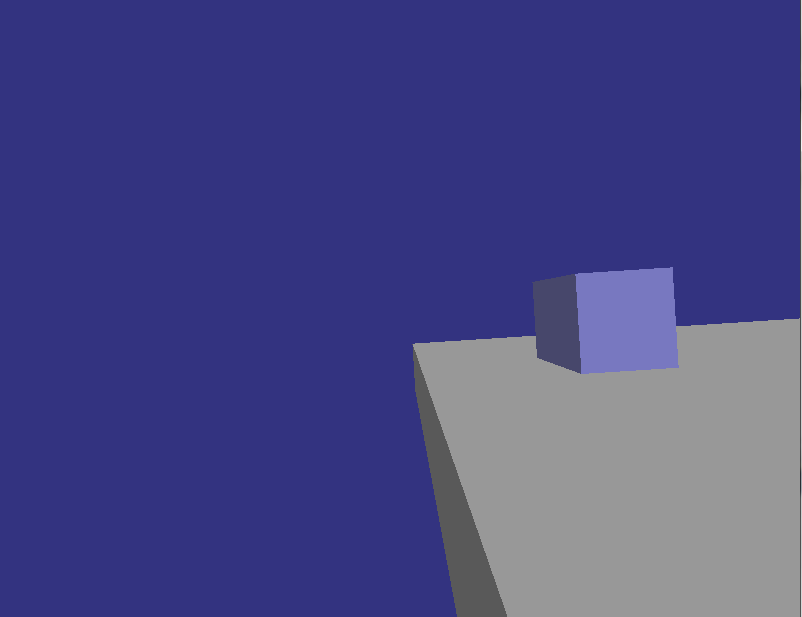
\includegraphics[width=.6\linewidth]{box_platform_a.png}}
	\label{fig:subfig1}
}
\subfigure {
	\fbox{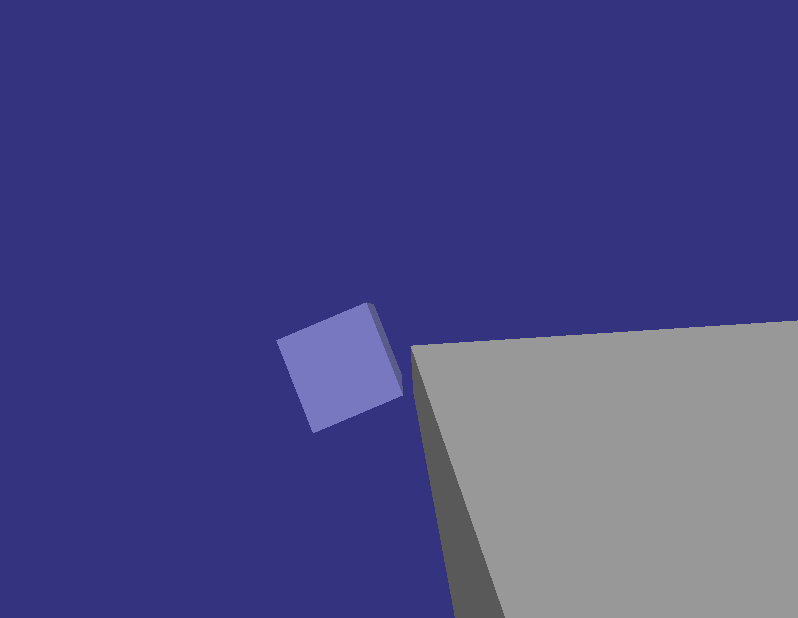
\includegraphics[width=.6\linewidth]{box_platform_b.png}}
	\label{fig:subfig2}
}
\caption{A box seen sliding down a plank smoothly at all times. }
\label{boxPlank}
\end{figure}

In the first scene (Figure~\ref{boxPlank}), we demonstrate the accuracy of the method with the box on plank scene. This scene can be viewed as an instance of Figure 3. As with the case of Figure 3 without culling non-admissible contact points/normals, a normal opposing the direction of the box sliding would prevent the box from sliding smoothly off of the edge of the plank as evident in the figure. \newline

\setlength\fboxsep{0pt}
\setlength\fboxrule{0.5pt}
\begin{figure}[ht]
\centering
\fbox{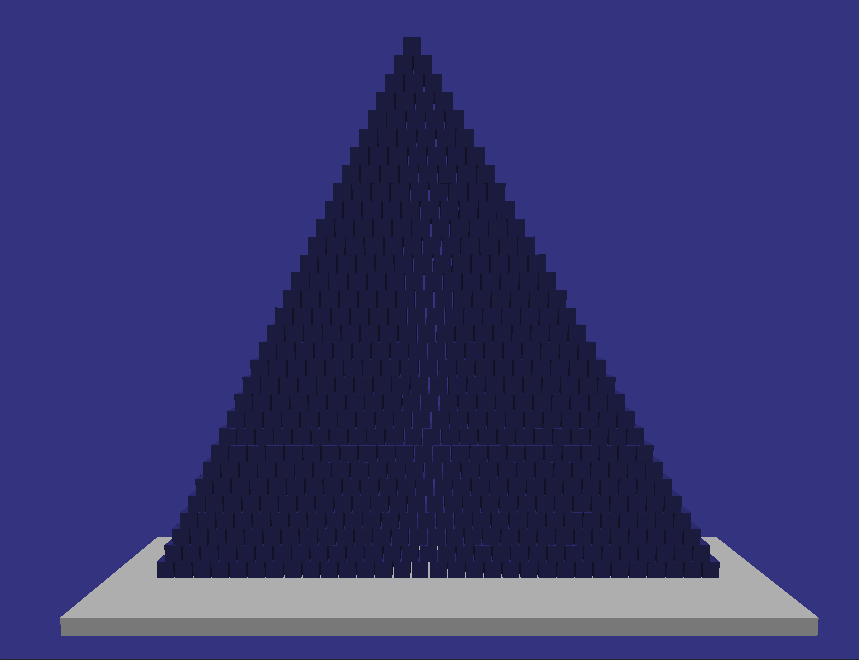
\includegraphics[width=\linewidth]{result_1.png}}
\label{boxPyramid}
\caption{Box-Pyramid}
\end{figure}

In the second scene (Figure 8), we consider a stable stack of 450 boxes that necessitates edge and face samples. In comparison to Bullet, it is seen that the collision detection phase is noticeably slower. This results from Bullet's implementation of GJK to cache contact points on the contact manifold, allowing for future GJK queries to run in nearly constant time. Although it is possible to cache contact points in our scheme, we wish to avoid the loss of accuracy incurred by a caching scheme, and we are mostly interested in simulating scenes that may have little temporal coherence. In terms of the constraint resolution phase, our phase is faster because of the fewer number of contact points as well as our implementation of the  projected Gauss-Siedel solver. This results in the overall simulation running faster than Bullet's; however, this purely due to the faster nature of constraint solving. \newline

\begin{figure}[ht]
\centering
\fbox{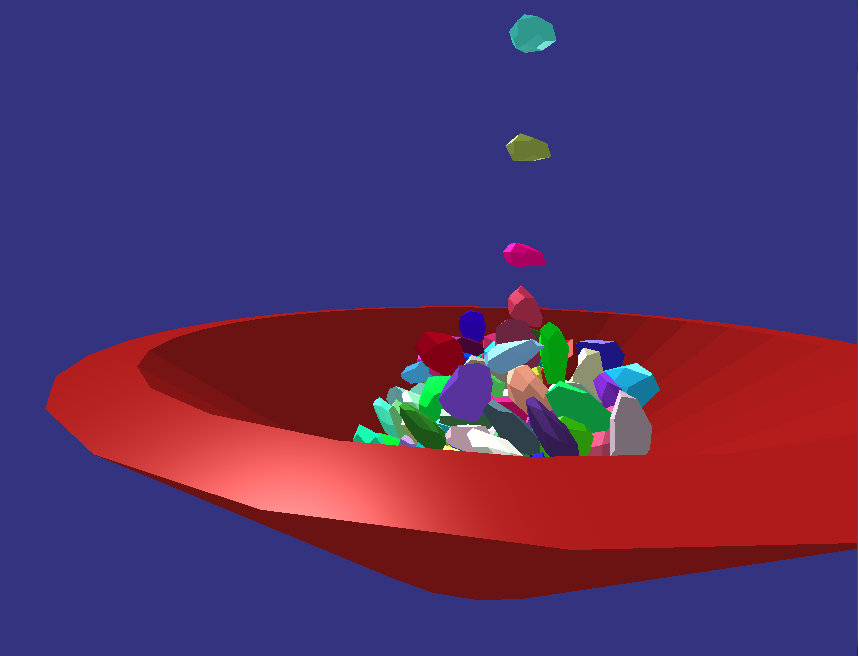
\includegraphics[width=\linewidth]{result_2.png}}
\label{Convex}
\caption{Convex}
\end{figure}

The third scene (Figure 9) shows 200 convex bodies being dropped into a funnel. The timing information is taken after the bodies have nearly all come to rest in the funnel. In our simulation and Bullet's, the collision detection phase dominates the simulation. Although Bullet's collision detection phase is faster than ours, the difference has become relatively small. The added cost to collision detection is due to the less stable nature of a pile of  bodies. In such a pile, the bodies will tend jitter slightly, invalidating cached contact points. \newline

\begin{figure}[ht]
\centering
\fbox{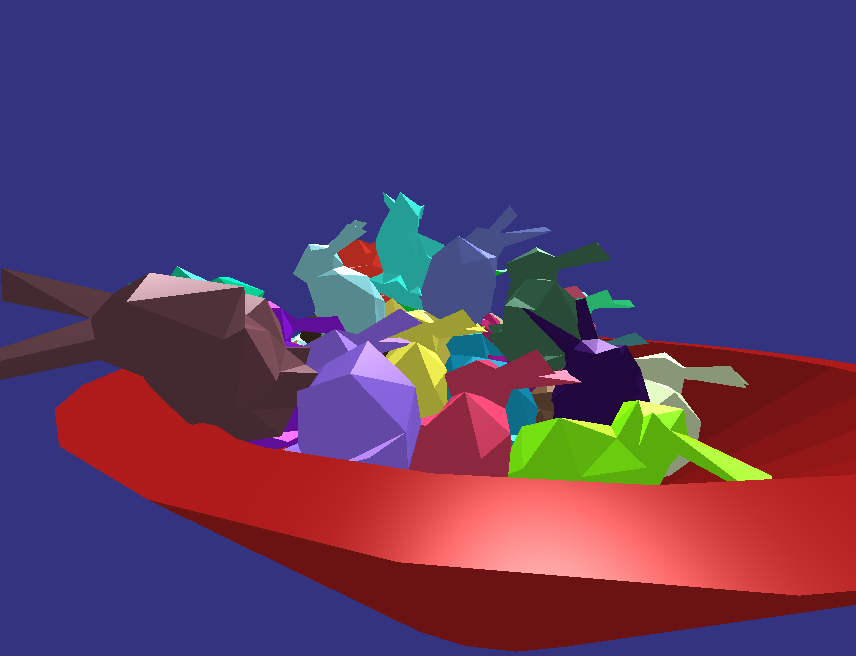
\includegraphics[width=\linewidth]{result_3.png}}
\label{concaveSimple}
\caption{Concave Simple}
\end{figure}

In the final scene (Figure 10), 50 coarsely tessellated Stanford Bunnies are dropped into the funnel. Like the prior scene, collision detection dominates the simulation; however, for this simulation, our method vastly outperforms Bullet for the collision detection phase. This is rather unsurprising since GJK must use a convex decomposed representation of the bunny of which there are many convex pieces. 

\section{Conslusion}

We have presented a new approach for the treatment of discrete collision detection. Our approach improves on the the method of signed distance fields to eliminate incorrect contact points/normals and handle efficiently and robustly the edge-edge and face-face contact cases. Our results demonstrate that our method is accurate and is nearly as fast for convex bodies and significantly faster for concave bodies compared to the GJK algorithm.

\begin{thebibliography}{9}

\bibitem{Allard} J. Allard, F. Faure, H. Courtcuisse. ``Volume Contact Constraints at Arbitrary Resolution.'' 
{\it SIGGRAPH '10 ACM SIGGRAPH 2010 Papers}, Article 42, pp. 1-10 (2010). 

\bibitem{Coumans} E. Coumans. ``Contact Generation.'' {\it GDC 2010}

\bibitem{English} R. E. English, M. Lentine, R. Fedkiw. ``Interpenetration Free Simulation of Thin Shell Rigid Bodies.'' {\it Transactions on Visualization and Computer Graphics.} pp. 1-14 (2012). 

\bibitem{ErlebenPhd} K. Erleben. ``Stable, Robust, and Versatile Multibody Dynamics Animation.'' PhD Thesis, Department of Computer Science, University of Copenhagen (DIKU), 2005.

\bibitem{Erlebenetal} Kenny Erleben, Jon Sporring, Knud Henriksen, Henrik Dohlmann, Physics Based Animation (Graphics). Cengage Learning; 1 edition (August 9, 2005).

\bibitem{Faure} F. Faure, S. Barbier, J. Allard, et al. ``Image-based Collision Detection and Response Between Arbitrary Volume Objects.'' {\it Eurographics/ACM SIGGRAPH Symposium on Computer Animation.} pp. 155-162 (2008). 

\bibitem{Gilbert} E. G. Gilbert, D. W. Johison, S. S. Keerth. ``A Fast Procedure for Computing the Distance Between Complex Objects in Three-Dimension Space.'' {\it IEEE Journal of Robotics and Automation}, Vol 4, No. 2, pp. 193-203 (April, 2008). 

\bibitem{Gottschalk} S. Gottschalk, M. C. Lin, D. Manocha ``OOBTree: A Hierarchical Structure for Rapid Interference Detection.'' {\it SIGGRAPH '96 Proceedings of the 23rd Annual Conference on Computer Graphics and Interactive Techniques}, pp. 171-180 (1996). 

\bibitem{Guendelman} E. Guendelman, R. Bridson, R. Fedkiw. ``Nonconvex Rigid Bodies with Stacking.'' {\it ProceedingSIGGRAPH '03 ACM SIGGRAPH 2003 Papers},pp. 871-878 (2003).

\bibitem{Heidelberger} B. Heidelberger, M. Teschner, M. Gross. ``Real Time Volumetric Intersections of Deforming Objects.'' {\it Proceedings of the Vision, Modeling, and Visualization Conference 2003} (Nov 2003). 

\bibitem{Hubbard} P. M. Hubbard. ``Collision Detection for Interactive Graphics Application.'' {\it IEEE Transations on Visualization and Computer Graphics}.Vol 1, Issue 3, pp. 218-230 (Sept 1995).

\bibitem{Lin} M. Lin, D. Manocha. ``Collision and Proximity Queries.'' {\it Handbook of Discrete and Computational Geometry: Collision Detection} Chapter 35, pp.1-21 (2003). 

\bibitem{Mirtich} Brian Mirtich. ``V-Clip: fast and robust polyhedral collision detection.'' \emph{ACM Transactions on Graphics (TOG)}, Volume 17 Issue 3, July 1998, 177-208.

\bibitem{Sethian} J. A. Sethian. ``A Fast Marching Level Set Method for Monotonically Advancing Fronts.''  {\it The Proceedings of the National Academy of Science of the United States of America} Vol 93, No 4, pp. 1591-1595 (1996).

\bibitem{Sud} A. Sud, N. Gooindaraju, D. Gayle, et al. ``Fast Proximity Computation Among Deformable Models Using Discrete Voronoi Diagrams.'' {\it ACM Transactions on Graphics (TOG) - Proceedings Of ACM SIGGRAPH 2006} Vol 25, Issue 3, pp. 1144-1153 (July 2006).

\bibitem{Teschner} M. Teschner, M. Kimmerle, B. Heidelberger, et al. ``Collision Detection for Deformable Objects.'' {\it Eurographics State-of-the-Art Report (EG-STAR}, Vol XX, No. X, 119-139 (2005). 

\bibitem{Tsitsiklis} J. N. Tsitsiklis. ``Efficient Algorithms for Globally Optimal Trajectories.'' {\it IEEE Transactions on Automatic Control}, Vol 4, No 2 (April 2008).

\bibitem{Vassilev} T. Vassilev, B. Spanglang, Y. Chrysanthou. ``Fast Cloth Animation on Walking Avatars.'' {\it EUROGRAPHICS - Computer Graphics Forum}, Vol 20, No. 3, pp. 260-276 (Sept 2001).

\bibitem{Wong} W. Wong, G. Baciu. ``GPU-based Intrinsic Collision Detection for Deformable Surfaces.'' {\it Computer Animation and Virtual Worlds}, Vol 16, Issue 3-4, pp. 153-161 (July 2005). 

\end{thebibliography}
\end{document}